\section{Re-Analyzing \texttt{Min-p}'s Human Evaluations}
\label{sec:human_evals}

We began with re-analyzing the original paper's human evaluations since human judgments are widely considered the gold standard for assessing language model outputs \citep{van2019best,roller2020opendomainconversationalagentscurrent,howcroft2020twenty,clark2021all,liang2022holistic,khashabi2022geniereproduciblestandardizedhuman,chiang2024chatbotarenaopenplatform,biderman2024lessonstrenchesreproducibleevaluation,schaeffer2025correlatingpredictinghumanevaluations}. 
We identified four key issues.

\subsection{Human evaluators’ scores for one of two baseline samplers were omitted}
\label{sec:human_evals:subsec:omitted_data}

Section 6 of \citet{nguyen2024minp} states human participants evaluated \texttt{min-p} against a single sampler: \texttt{top-p}.
Both the \href{https://arxiv.org/abs/2407.01082v2}{Oct 2024 Arxiv manuscript} and \href{https://openreview.net/notes/edits/attachment?id=SR6ORZeBAn&name=pdf}{ICLR OpenReview manuscript} repeatedly state that \texttt{min-p} and \texttt{top-p} were considered, and their Table 4 presents results only for these.
However, when examining the \href{https://github.com/menhguin/minp_paper/blob/main/min_p%20user%20preference%20study%20v2.0%20(Responses)%20-%20Form%20responses%201%20(1)%20(2).csv}{paper's data}, we discovered that \textbf{scores for a second baseline sampler (\texttt{basic} sampling) were excluded from the methodology, the analysis and the results without mention or explanation}. 
We \href{https://github.com/menhguin/minp_paper/issues/4}{publicly confirmed with the authors}.
These omitted scores comprised $1/3^{\text{rd}}$ of the total collected scores.
After we raised the issue, the omitted data were added to the \href{https://openreview.net/notes/edits/attachment?id=oQLYV9wuaa&name=pdf}{Camera Ready's Table 4}, but the methodology, the results and the conclusions have not been correspondingly updated.

\begin{figure}[t!]
    \centering
    \begin{minipage}{\textwidth}
        \centering
        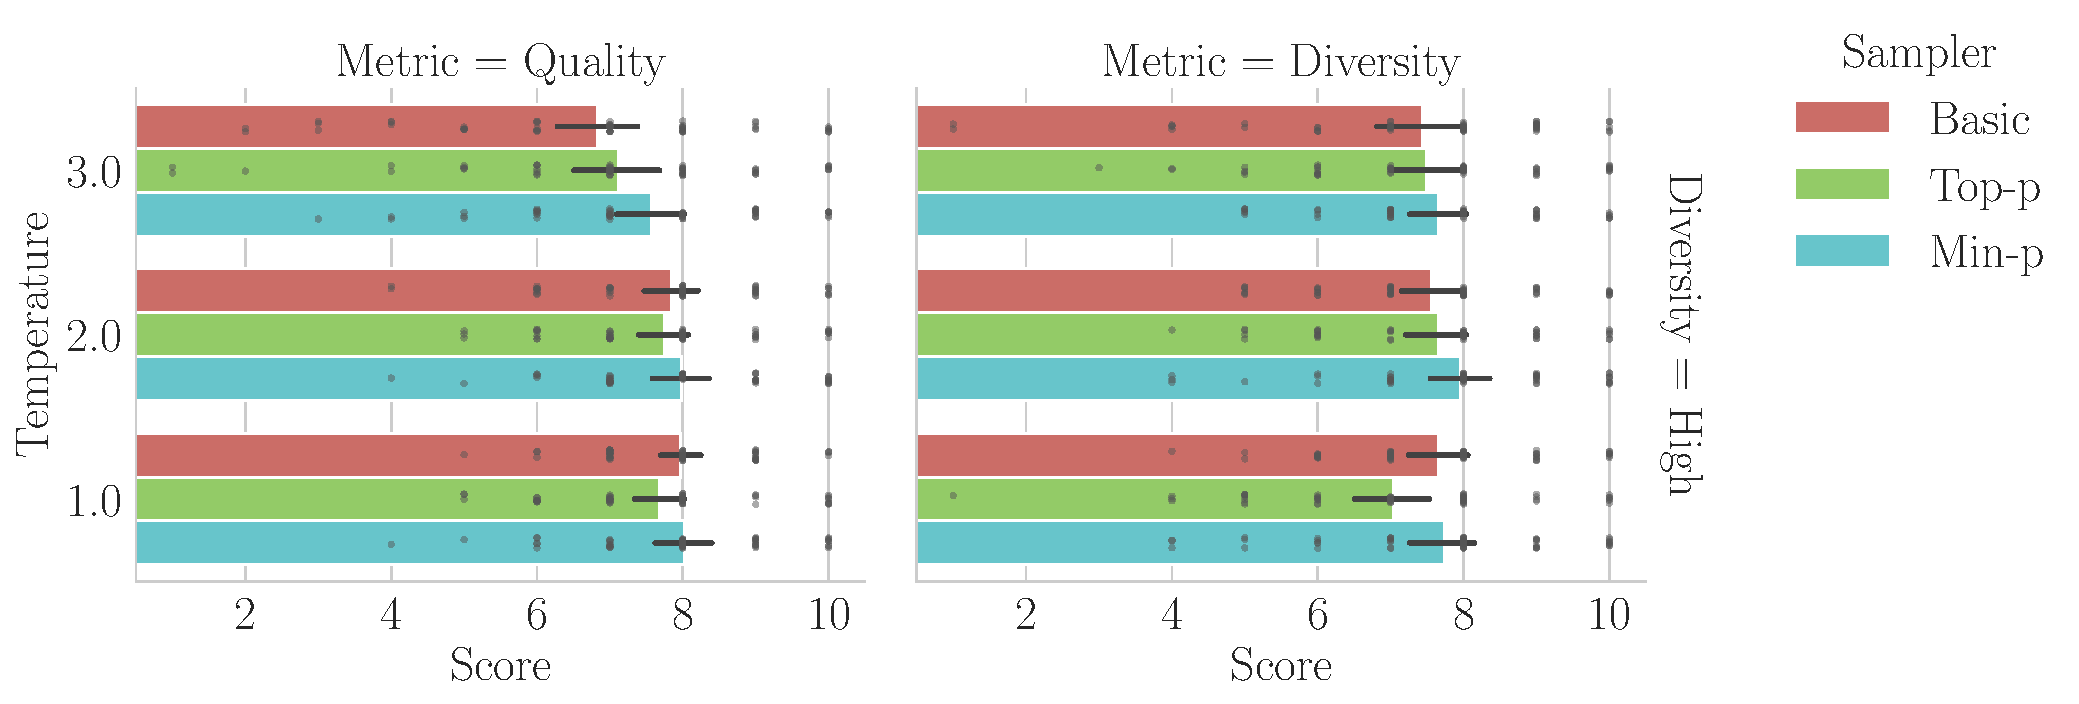
\includegraphics[width=\linewidth]{figures/human_evals/attentive_y=temp_x=score_hue=sampler_row=diversity_col=metric_barnstrip.pdf}
        \captionof{figure}{\textbf{Visualizing Human Evaluators' Scores from \citet{nguyen2024minp}'s Data Demonstrates \texttt{Min-p} Does Not ``Consistently" Outperform Other Samplers.} Rather, the original paper's data suggest \texttt{min-p} is largely indistinguishable from other samplers based on 95\% confidence intervals.}
        \label{fig:human_evals}
    \end{minipage}
\end{figure}


\subsection{Visualizations and Statistical Tests Fail to Support Claim That \texttt{Min-p} Outperforms Other Samplers}
\label{sec:human_evals:subsec:human_scores}

Based on the human evaluators' scores, Section 6 of \citet{nguyen2024minp} concluded that \texttt{min-p} ``consistently" outperformed \texttt{top-p} ``across all settings":
%
\begin{quote}
    ``Overall, \texttt{min-p} sampling consistently scored higher than \texttt{top-p} sampling across all settings [...] A paired t-test confirmed that the differences in scores between min-p and top-p sampling were statistically significant ($p < 0.05$).''
\end{quote}
%
However, \textbf{both visualizations and statistical hypothesis tests of the original human evaluation data suggest \texttt{min-p} is indistinguishable from the baselines in almost all settings.}

To briefly explain the human evaluation methodology, three samplers (\texttt{basic}, \texttt{top-p} and \texttt{min-p}) were compared in six conditions: three temperatures ($1.0, 2.0, 3.0$) and two diversity settings (``high" and ``low") corresponding to different $p$ hyperparameters.
Humans were asked to score the generated outputs under two metrics: quality and diversity.
Participants were excluded if they failed attention checks.
For more information, please see the original manuscript.

\begin{table}[t!]
    \centering
    % Paired t-test Results Table
    \begin{tabular}{llcccccc}
    \toprule
    \multirow{2}{*}{Metric} & \multirow{2}{*}{Alt. Hyp.} & \multicolumn{6}{c}{Temperature} \\
    \cmidrule(lr){3-8}
    & & \multicolumn{2}{c}{$\tau=1.0$} & \multicolumn{2}{c}{$\tau=2.0$} & \multicolumn{2}{c}{$\tau=3.0$} \\
    \cmidrule(lr){3-4} \cmidrule(lr){5-6} \cmidrule(lr){7-8}
    & & $t$ & $p$ & $t$ & $p$ & $t$ & $p$ \\
    \midrule
    \multirow{2}{*}{Quality} & \texttt{Min-p} $>$ \texttt{Basic} & 0.33 & .370 & 0.65 & .260 & 3.13$^{***\dagger}$ & .001 \\
    & \texttt{Min-p} $>$ \texttt{Top-p} & 2.05$^{*}$ & .023 & 1.18 & .121 & 2.02$^{*}$ & .025 \\
    \midrule
    \multirow{2}{*}{Diversity} & \texttt{Min-p} $>$ \texttt{Basic} & 0.31 & .378 & 1.86$^{*}$ & .034 & 0.85 & .201 \\
    & \texttt{Min-p} $>$ \texttt{Top-p} & 2.64$^{**}$ & .006 & 1.44 & .078 & 0.87 & .195 \\
    \bottomrule
    \multicolumn{8}{l}{\scriptsize{$^{*}$ $p < 0.05$, $^{**}$ $p < 0.01$, $^{***}$ $p < 0.001$, $^{\dagger}$ Significant after Bonferroni correction for 12 comparisons.}} \\
    \multicolumn{8}{l}{\scriptsize{Note: All tests were paired t-tests with df = 52, one-sided (alternative = "greater")}} \\
    \phantom{Blank Line}\\
    \end{tabular}\\
    \captionof{table}{\textbf{Hypothesis Testing of Human Evaluators' Scores Fails to Support Claim that \texttt{Min-p} Consistently Outperforms Other Samplers.} To test whether evidence supports the claim that \texttt{min-p} ``consistently outperforms" other samplers, we conducted one-sided paired t-tests using the authors' published data. Without correcting for multiple comparisons, evidence exists to support \texttt{min-p}'s superiority in 5 of 12 comparisons at $\alpha=0.05$ and 2 of 12 comparisons at $\alpha=0.01$. After applying a Bonferroni correcting for multiple comparisons, evidence exists to support \texttt{min-p}'s superiority in 1 of 12 comparisons at $\alpha=0.05$ and 0 of 12 comparisons at $\alpha=0.01$. For details, see Sec.~\ref{sec:human_evals:subsec:human_feedback}.}
    \label{tab:human_evals_paired_ttests}
\end{table}

We focused on the ``high" diversity setting for three reasons: 
First, the claimed advantage of \texttt{min-p} sampling is that it provides both high quality and high diversity, whereas other samplers typically trade one off against the other. Second, \href{https://github.com/menhguin/minp_paper/issues/4}{the authors publicly told us to focus on the high diversity setting}, writing that ``the low [diversity] settings were quite experimental". Third, we believe that \texttt{top-p}'s $p$ value in the low diversity setting was poorly chosen; indeed, after we raised these concerns, the authors ran a new human evaluation that changed the low diversity \texttt{top-p} $p$ from $0.1$ to $0.9$. We return to this second new human evaluation in Sec.~\ref{sec:human_evals:subset:new_exp}.

We began by visualizing the human evaluations' scores from \citet{nguyen2024minp}. \textbf{Using the original paper's data, Fig.~\ref{fig:human_evals} reveals that the three samplers provide similar quality and similar diversity, with 95\% confidence intervals frequently overlapping}.

To more rigorously assess the claim that \texttt{min-p} consistently outperforms other samplers, we conducted 12 one-sided paired t-tests for each metric (quality or diversity), temperature ($1.0, 2.0, 3.0$) and baseline sampler (\texttt{min-p} versus \texttt{basic}, \texttt{min-p} versus \texttt{top-p}). In each test, the null hypothesis is \texttt{min-p}'s score is less than or equal to the other sampler's score, and the alternative hypothesis is \texttt{min-p}'s score is greater than the other sampler's score.
Statistical test results are displayed in Table~\ref{tab:human_evals_paired_ttests}.
Without correcting for multiple comparisons, we found evidence to reject the null hypotheses in 5 of 12 tests at $\alpha=0.05$ and 2 of 12 tests at $\alpha=0.01$. After applying a Bonferroni correction for multiple comparisons, we found evidence to reject the null hypothesis in 1 of 12 tests at $\alpha=0.05$ and 0 of 12 tests at $\alpha=0.01$.
\textbf{Based on the original paper's data, there is insufficient evidence to support the claim that \texttt{min-p} consistently outperforms baseline samplers across all settings.}

Furthermore, given that the original paper claims that \texttt{min-p} ``consistently" scores higher, an Intersection-Union Test (IUT) may be the appropriate statistical test, where the alternative hypothesis is that \texttt{min-p} is better in all 12 comparisons and the null hypothesis is the set complement. Since the largest p-value of the 12 comparisons is $0.378$, under the IUT, we again find insufficient evidence to reject the null hypothesis at both $\alpha=0.05$ and $\alpha=0.01$.

The original paper's statistical analysis reached a different conclusion for two reasons. First, despite claiming that \texttt{min-p} ``consistently scored higher" ``across all settings"  (metric, temperature, and diversity), the paper pooled data across all settings and performed a single t-test, which tests whether \texttt{min-p} scored higher on average. Second, pooling over all settings is misleading in that in the ``low'' diversity condition, \texttt{top-p}'s hyperparameter $p$ was poorly chosen in a way that pulled \texttt{top-p} down significantly; the authors said publicly to ignore this particular low diversity condition and subsequently changed $p$ in their new human experiment (Sec.~\ref{sec:human_evals:subset:new_exp}).
Thus, we believe the original paper's statistical inferences are misleading or incorrect.

\subsection{Human Evaluators' Qualitative Responses Fail to Support Claim That \texttt{Min-p} Is Preferred Over Other Samplers}
\label{sec:human_evals:subsec:human_feedback}

\begin{figure}[t!]
    \centering
    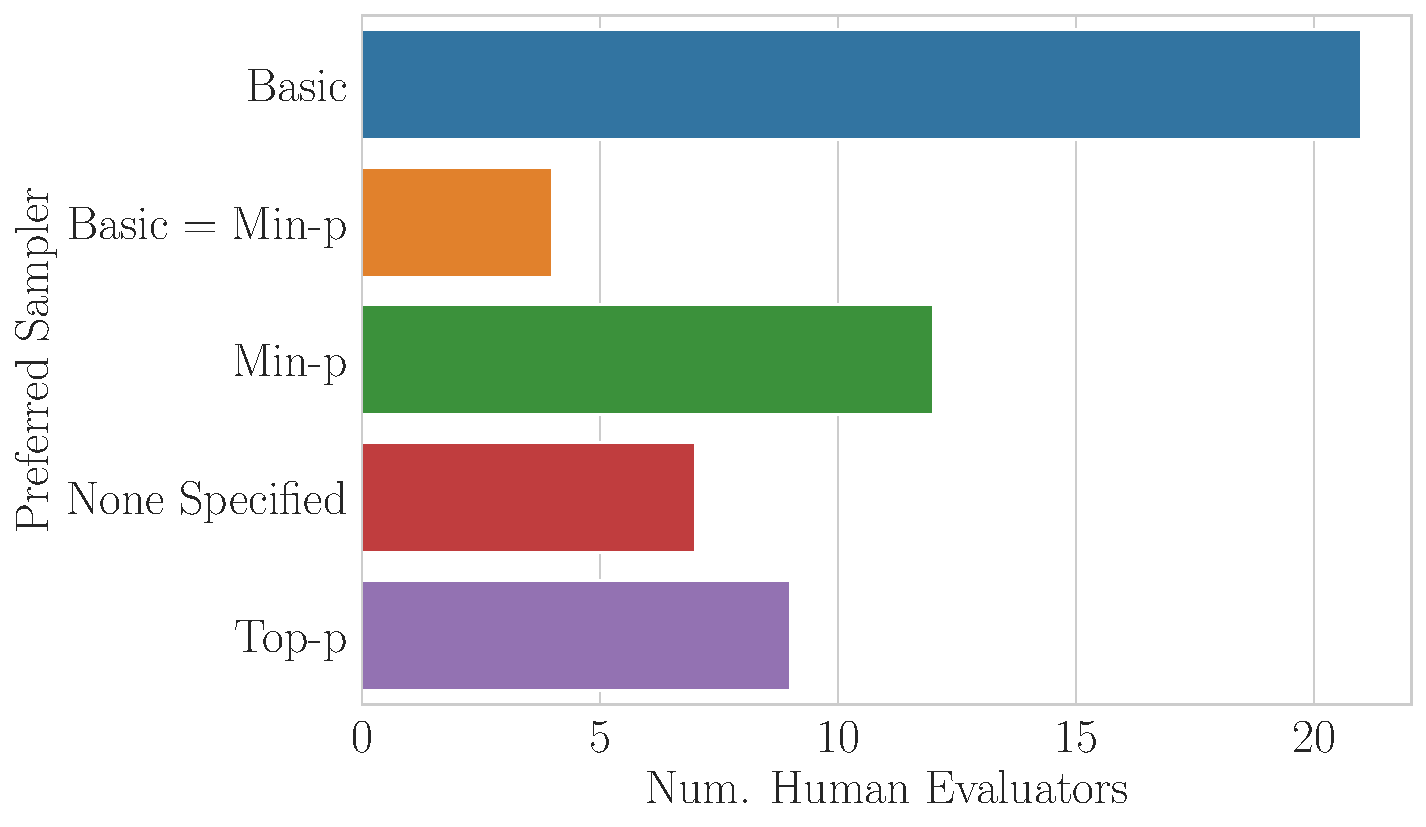
\includegraphics[width=0.7\linewidth]{figures/human_evals/attentive_human_annotators_preferred_samplers.pdf}
    \caption{\textbf{Manual Annotation of Human Evaluators' Qualitative Responses Fail to Support Claim that \texttt{Min-P} Was the Preferred Sampler.} We manually annotated responses from human annotators regarding their preferred sampler(s) at the end of the original paper's study. The responses suggest \texttt{min-p} was not the most preferred sampler. We provide example responses in Sec.~\ref{sec:human_evals:subsec:human_feedback}.}
    \label{fig:attentive_human_annotators_preferred_samplers}
\end{figure}


At the end of the human evaluation study, the original paper asked human participants to qualitatively describe which sampler(s) they preferred. The paper claimed that human evaluators' qualitative responses support \texttt{min-p} over \texttt{top-p}:
%
\begin{quote}
    ``Participants frequently noted that outputs generated with min-p sampling were more coherent and creative, especially at higher temperatures.''
\end{quote}
%
However, when reading through the  \href{https://github.com/menhguin/minp_paper/blob/main/min_p%20user%20preference%20study%20v2.0%20(Responses)%20-%20Form%20responses%201%20(1)%20(2).csv}{paper's data}, we believe that \textbf{the qualitative responses suggest a different preference pattern}.
We manually annotated the qualitative responses and visualized our annotations of the humans' expressed preferences (Fig.~\ref{fig:attentive_human_annotators_preferred_samplers}), and \href{https://docs.google.com/spreadsheets/d/1-KNh4-dbrXBafb9iUQINqFBjDrZvkScPNbGH6IENecQ/edit?gid=1288914057#gid=1288914057}{publicly posted our annotations} in the same format as the original paper.
We found two results: (1) more human evaluators explicitly preferred \texttt{basic} sampling than preferred \texttt{min-p} sampling, and (2) \texttt{min-p} was only slightly preferred over \texttt{top-p}.
We provide quotations from human evaluators favoring \texttt{basic} sampling in Appendix~\ref{app:sec:human_qual_responses}.

\subsection{New Human Evaluation Study Shows \texttt{Min-p} Does Not Outperform Baselines in Quality, in Diversity, or in a Tradeoff Between Quality and Diversity}
\label{sec:human_evals:subset:new_exp}

In response to our feedback, the authors conducted and added a new human evaluation study to Appendix C.2.
Their new study made multiple methodological changes:
%
\begin{itemize}
    \item Different sampler implementation: switched from applying temperature \textit{after} truncation to applying temperature \textit{before} truncation.
    \item Different distribution of human participants from Prolific.
    \item Different sampling hyperparameters for \texttt{top-p}: switched from $0.1$ and $0.9$ to $0.9$ and $0.95$.
    \item Different sampling hyperparameters for \texttt{min-p}: switched from $0.2$ and $0.05$ to $0.1$ and $0.05$.
    \item Different allotted reading time: increased from 30 minutes to 45 minutes.
    \item Different sampled text: 3 short paragraphs were replaced with a single complete story.
    \item Different rubric for human participants to evaluate sampled outputs.
\end{itemize}
%
Regarding the \href{https://github.com/menhguin/minp_paper/blob/main/%5BLIVE%5D%20min_p%20user%20preference%20study%20v3.0%20(Responses)%20-%20Form%20responses%201.csv}{new human evaluation data} and results, we share two discoveries here: First, we believe one value is incorrectly reported: in \citet{nguyen2024minp}'s Table 15, the average score of \texttt{min-p} at $p=0.05$ and temperature $T=2$ is reported as $7.80$, but based on the authors' publicly posted data, we believe the correct numerical value should be $5.80$. Second, more generally, the data show again that \texttt{Min-p} does not outperform baselines in quality, in diversity or in a favorable tradeoff between quality and diversity. In this new study, whenever \texttt{min-p} outperforms other samplers, it does so under conditions that yield lower absolute scores than other conditions (Fig.~\ref{fig:new_human_evals}). For instance, \texttt{min-p} shows an advantage over the baselines in the ``high" diversity setting at $T=2$ and in the ``low" diversity setting at $T=3$. However, in both of these conditions, \texttt{min-p} receives lower quality and diversity scores than it does in the ``high" diversity setting at $T=1$ and the ``low" diversity setting at $T=2$. This shows \texttt{min-p}'s advantage is observed primarily under conditions that yield lower overall quality and diversity scores compared to other achievable conditions. \textbf{For anyone seeking higher quality or diversity, \texttt{min-p} offers no apparent advantage over \texttt{basic} or \texttt{top-p} sampling}.

\begin{figure}[t!]
    \centering
    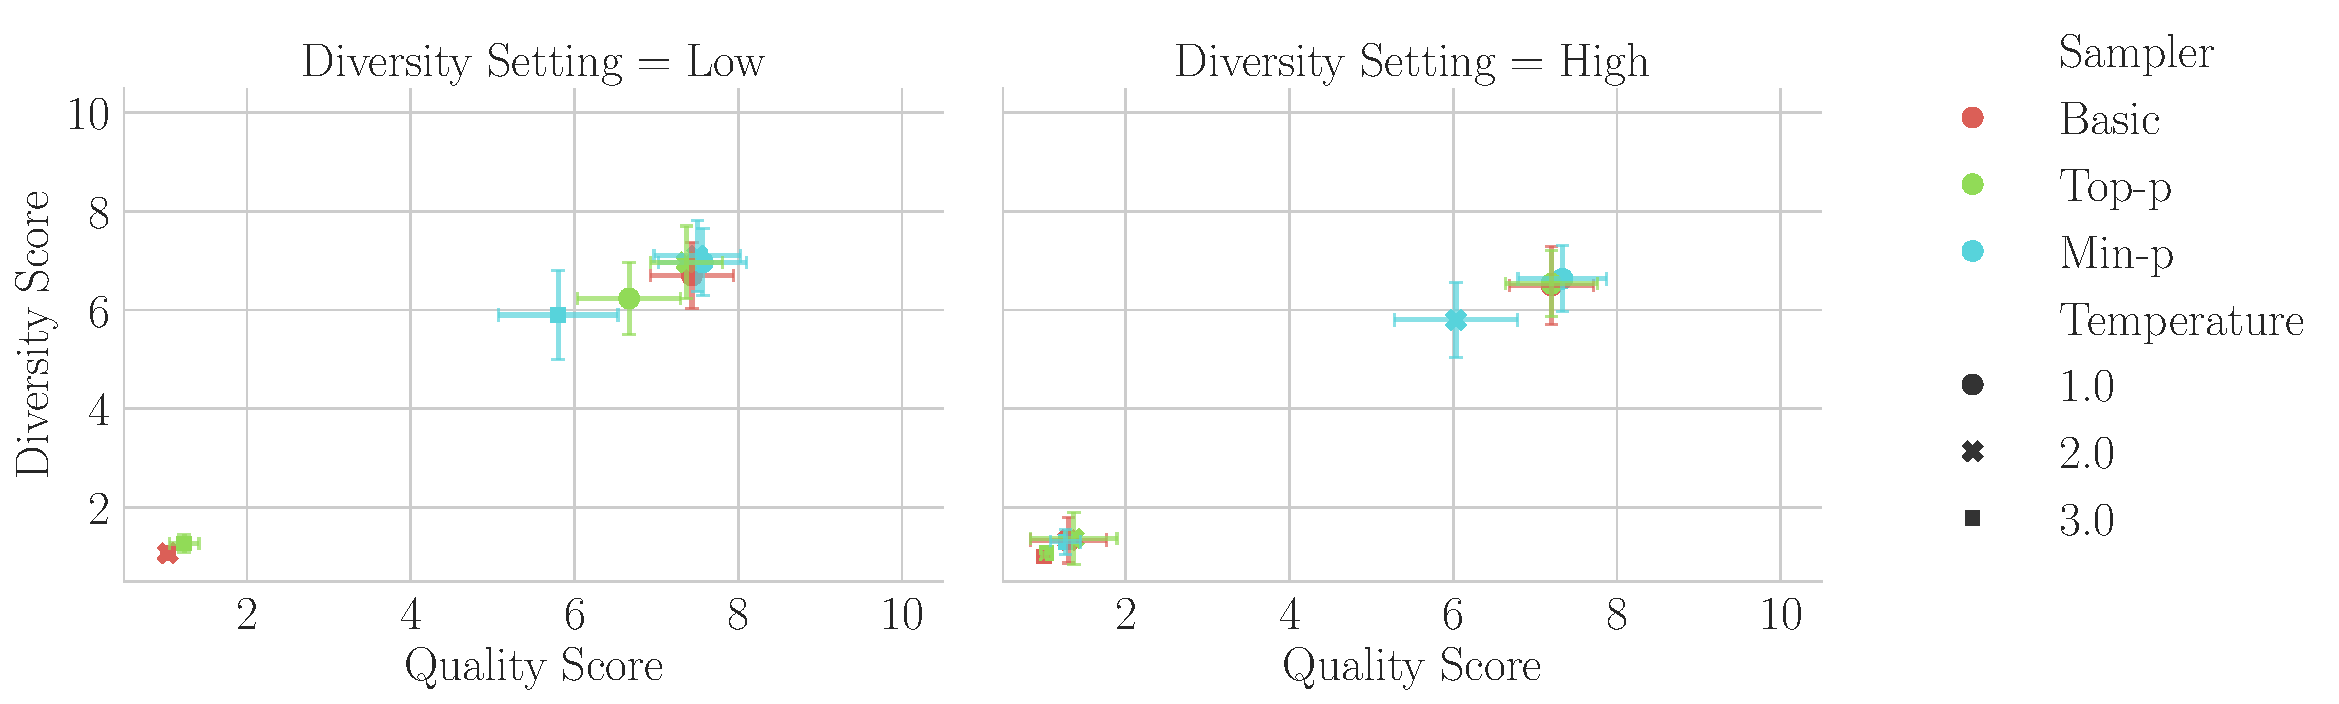
\includegraphics[width=\linewidth]{figures/new_human_evals/attentive_y=diversity_score_x=quality_score_hue=sampler_col=diversity_style=temp.pdf}
    \captionof{figure}{\textbf{New Human Evaluation Study Suggests \texttt{Min-p} Does Not Outperform Baselines in Quality, in Diversity or in a Pareto-Optimal Tradeoff Between Quality and Diversity.} Visualization of scores from \citet{nguyen2024minp}'s second human experiment. \texttt{Min-p}'s performance advantage relative to \texttt{basic} and \texttt{top-p} sampling is observed in conditions (e.g., higher temperatures) where absolute quality and absolute diversity scores across all samplers are lower compared to other regimes (e.g., $T=1$). For practitioners optimizing for maximal quality and maximal diversity, these results suggest that \texttt{min-p} offers no apparent advantage over \texttt{basic} or \texttt{top-p} sampling.}
    \label{fig:new_human_evals}
\end{figure}